\documentclass[12pt,fleqn]{jsotsuron}
\setlength{\mathindent}{2zw}
\usepackage[dvipdfmx]{graphicx}
\usepackage{makeidx}
\usepackage{amsmath,amssymb}
\usepackage{amsthm}
\usepackage{algorithmic}
\usepackage{algorithm}
\usepackage{url}
\usepackage{here}
\renewcommand{\algorithmicrequire}{\textbf{Input:}}
\renewcommand{\algorithmicensure}{\textbf{Output:}}
\renewcommand{\proofname}{証明}
\newtheorem{Theorem}{定理}
\newtheorem{Definition}{定義}
\newtheorem{Proof}{証明}[section]
\renewcommand{\proofname}{証明}
\renewcommand{\theProof}{}
\newtheorem{Lemma}{命題}[section]
\def\vector#1{\mbox{\boldmath $#1$}}
\bibliographystyle{jplain} 

\title{Wildcardを許容した頻出部分グラフ列挙とその出力要約\\
``Frequent Subgraph Mining with Wildcards and its Output Summarization''}
\author{岡崎 文哉}
\date{平成28年2月}
\makeindex

\begin{document}
\maketitle
\tableofcontents
\newpage

\chapter{はじめに}
\section{背景}
データマイニングや知識発見の主要な研究題目のひとつである
頻出パターンマイニングは,データベース中に高頻度に存在する
パターンをすべて列挙する問題である.
その対象はアイテムセット,文字列,木やグラフで表される多種多様な構造を含む.
グラフデータベースから頻出する部分グラフパターンを発見する問題は,
化合物データベース,タンパク質-タンパク質ネットワーク,XML文節データベース
などのグラフデータベースから特徴的な部分構造を見つける多くの応用が
存在するため,これまでデータマイニングの分野で,
いくつものグラフマイニングアルゴリズムが提案されている
(FSSM\cite{fssm},FSG\cite{fsg},AGM\cite{agm1,agm2},
gSpan\cite{gSpan},Gaston\cite{gaston}).

扱うグラフデータベースでは辺や頂点にラベルが与えられており,
頻出部分グラフマイニングにより見つかる部分グラフには
一部のラベルが異なるだけの類似部分グラフが多数存在する.
従ってラベルを区別しないwildcardラベルを含んだ部分グラフを求めることで,
よりデータの構造を反映した柔軟なパターンが発見できると考えられる.
一般的にwildcardは文字列検索などの際に指定する特殊文字の1種で,
どのような文字・文字列にもマッチするものとして扱われるが,
本研究でにおいてwildcardは出現パターン
において辺や頂点のどのようなラベルにもマッチするラベルとして扱う.

関連研究として,化学の分野において化合物におけるwildcardの有用性の研究がある.
Hoferら\cite{wildcard}は化学の分野において同様の働きをしているとみなした
複数の種類の頂点をwildcardとして処理をすることで有用なパターンを見つけること
ができたとしている.また,文字列における頻出パターンマイニングにおいてwildcard
を考慮した研究\cite{ws1,ws2,ws3}も存在する.マイニングとは異なるが,グラフの検索
\cite{graphgrep,graphfind}の分野でもwildcardを含むグラフを検索する研究もある.
しかしマイニングの分野では頻出部分グラフマイニングにおける全列挙という点で既存研究はほぼ見受けられない.その一つの理由としてwildcard導入による出力パターン数の劇的な増大が実用を妨げる点があるものと思われる.

\section{概要}
本研究では,我々はwildcardを許容する部分グラフパターンが,
化合物データのみならず様々な
分野で有用であると考えた.頻出部分グラフマイニングに
wildcardを許容することで列挙される部分グラフ数が膨大に増加する問題の解決のために,
頻出パターンマイニングにおいてパターン集合要約に用いられる
飽和パターン集合・極大パターン集合を用いることができる.
そこで,頻出部分グラフマイニングにおいてwildcardを許容した部分グラフを
全列挙したうえで,膨大に増加するパターン集合を要約するため
飽和パターン集合と極大パターン集合を求める方法を提案する.
実験により,wildcardを許容することによる頻出パターン数の増加,および,飽和パターン・極大パターンによるパターン集合要約の効果を検証する.
さらに,wildcardを許容した頻出部分グラフを特徴として
グラフ分類を行うことで,wildcardを許容した頻出部分グラフが
どれほど有効であるかを実験し,考察する.

\section{構成}
本論文では,前節の概要について,以降の章で以下の通り詳述する.
\begin{itemize}
\item 第2章では,頻出部分グラフマイニングの記法,定義について述べる.
\item 第3章では,提案アルゴリズムのベースとなる既存手法を説明する.
\item 第4章では,wildcardを許容した頻出部分グラフマイニングへの拡張を提案する.
\item 第5章では,wildcardを許容した頻出部分グラフマイニングで求めた
パターン集合を要約し飽和パターン集合と極大パターン集合を求める手法を提案する.
\item 第6章では,提案した手法の実験結果を示す.
\item 第7章では,結論と,本研究の今後の展望を述べる.
\end{itemize}


\chapter{頻出部分グラフマイニング}

本章では,本研究で扱う頻出部分グラフマイニングについて説明する.

\section{グラフマイニング}
グラフマイニングとは,グラフを対象としたデータマイニングを指す.
化学式,WWWや社会ネットワークなどグラフで表される幅広い応用が存在する
ため,これまでにさまざまな研究が存在する.
グラフマイニングにおける重要な課題のひとつが,
本研究で扱う頻出部分グラフマイニングである.

頻出パターンマイニングは,データ集合中で,一定頻度以上現れるパターンを
列挙する手法である.頻出パターンマイニングにおける列挙の対象と
なるパターンは様々で,アイテムセットや系列データ,時系列,パス,部分木,部分グラフ
などが挙げられる.
本研究で扱う頻出部分グラフマイニングは,
頻出パターンマイニングにおける部分グラフ
を対象とした問題である.

\section{グラフの定義}

%このようなグラフ$G$は頂点集合を$V$,辺の集合を$E$,ラベル集合を$L$,$V\cup E$ からそのラベルへの写像を$l$とすると$G=(V,E,L,l)$と表すことができる.
\begin{Definition}[無向グラフ]
無向グラフは,頂点と呼ばれる要素の有限集合$V$,辺と呼ばれる要素の有限集合$E$,関数$\psi : E \rightarrow \{X ⊆ V |\ |X| = 2\} $
の3つの組$(V, E, \psi)$ で定義され,グラフ$G$の頂点集合や辺集合を$V(G),E(G)$と表し,$G=(V(G),E(G))$
とも書く.
\end{Definition}

本研究においてグラフは無向グラフを表しており,有向グラフについては考慮しない.

\begin{Definition}[部分グラフ]
2つのグラフ$G=(V(G),E(G))$に対して,
$V(G^{\prime })\subset V(G)$かつ$E(G^{\prime })\subset E(G)$となる
$G^{\prime } =(V(G^{\prime }),E(G^{\prime }))$が与えられたとき,
$G^{\prime }$を$G$の部分グラフと呼ぶ.
\end{Definition}

本研究で扱うグラフでは,多重辺や自己ループを含まず,
頂点・辺にラベルが付与された無向グラフとし,
本研究(および従来研究)での列挙対象は連結な部分グラフである.

\section{問題定義}
頻出部分グラフマイニングとは,グラフデータセット
$GS=\{G_i \mid i=1,2,3,\ldots ,n\}$に対して,
閾値$\sigma$が与えられた時,
%最小支持度(以下,minsup)が与えられた時,
ある部分グラフ$g$の支持度(以下,support)
$\mathrm{support}(g)=|\{G_i \mid G_i\in GS,gが
G_iのある部分グラフに同型\}|$について
$\mathrm{support}(g)\geq \sigma$となる部分グラフ$g$を
全列挙するという問題である.この指定される閾値$\sigma$を最小支持度
(以下,minsup)と呼ぶ.
頻出部分グラフマイニングは部分グラフ同型問題に密接に関係している.
部分グラフ同型問題の計算複雑さはNP完全であり,
この問題を効率よく解くアルゴリズムは知られていない\cite{gi}が
頻出部分グラフマイニングは前述したように実データの特性を活かして
高速に処理できるアルゴリズムが開発されている.
%実データ上では解くことのできるアルゴリズムが開発されている.

\section{既存手法}
%(FSSM\cite{fssm},FSG\cite{fsg},AGM\cite{agm1,agm2},AcGM\cite{acgm},
%gSpan\cite{gSpan},Gaston\cite{gaston})
%本節では,この論文にて用いたgSpanアルゴリズムについて説明する.
YanとHanにより開発されたgSpan\cite{gSpan}は,深さ優先探索木を拡張した
グラフマイニングアルゴリズムであり,
AGM\cite{agm1,agm2}やFSG\cite{fsg}のような隣接行列に基づいたApriori風の探索を行わず,
パターングラフを深さ優先で探索する点を特徴とし,メモリ効率がよい.
また,グラフ上の深さ優先探索により求められるDFSコードという符号をグラフの表現として用いる.
\subsection{DFSコード}
$G$を頂点の数が$k$のパターングラフとする.
まず,$G$の頂点を$1$から$k$まで番号をつけながら深さ優先探索を行い,
未探索の頂点に向かう辺をforward edge,探索済みの頂点に向かう辺をbackward edgeと呼ぶ.
ここで,$E^f$を$G$のforward edgeの集合,$E^b$を$G$のbackward edgeの
集合と表記する.
$T$の辺全体$E=E^f\cup E^b$上の
2項関係$\prec_T$を以下のように定義する.

任意の$e_1,e_2\in E$に対して,$e_1=(i_1,j_1),e_2=(i_2,j_2)(i_1,i_2,j_1,j_2は頂点番号)$とおくと,
$e_1\prec_T e_2$が成り立つのは以下の条件が成り立つときである.
\begin{enumerate}
\renewcommand{\labelenumi}{(\roman{enumi})}
  \item $e_1,e_2\in E^f$のとき,$j_1 < j_2$
  \item $e_1,e_2\in E^b$のとき,$i_1 < i_2またはi_1=i_2\wedge j_1 < j_2 $
  \item $e_1\in E^b,e_2\in E^f$のとき,$i_1 < j_2$
  \item $e_1\in E^f,e_2\in E^b$のとき,$j_1\leq i_2$
\end{enumerate}
2項関係$\prec_T$は$E$上の全順序になる.
本研究において$G$は辺ラベルをもつとしているため,
$e=(i,j)\in E$の符号を$e=(i,j,\mathrm{label}_i,\mathrm{edgelabel}_{i,j},\mathrm{label}_j)$とする.

Gの深さ優先探索順1つに対しDFSコードが一意に決まり,
$\mathrm{code}(G)=(e_1,e_2,\dots ,e_k)$(ただし$e_1\prec_T \dots \prec_T e_k$)と表せる.

\subsection{DFS辞書順}
あるグラフにおいて深さ優先探索順は多数存在するため,ここではそれぞれのDFSコードに辞書的順序を与えるためDFSコードの線形順序を定義する.
まずグラフ$G$に対して考えられるDFSコードすべての集合を$Z$とする.
任意の2つのDFSコード$\alpha = (a_0,a_1,\dots ,a_m)$,
$\beta = (b_0,b_1,\dots ,b_n)$,$\alpha ,\beta \in Z$が与えられた時,
DFS辞書順$\alpha \leq \beta$となるための条件は以下のどちらかを満たすときである.

\begin{enumerate}
\renewcommand{\labelenumi}{(\roman{enumi})}
  \item $\exists t,0\leq t\leq \mathrm{min}(m,n),0\leq k<tであるkについてa_k=b_kかつa_t\prec_eb_t$
  \item $0\leq k\leq mであるkについてa_k=b_kかつn\geq m$
\end{enumerate}

ここで使用した$a_t\prec_eb_t$が成り立つのは,
$a_t=(i_a,j_a,l_{i_a},l_{i_a,j_a},l_{j_a}),b_t=(i_b,j_b,l_{i_b},l_{i_b,j_b},l_{j_b})$
としたとき,以下のいずれかが成り立つときである.
\begin{enumerate}
\renewcommand{\labelenumi}{(\roman{enumi})}
  \item $a_t\in E_\alpha^bかつb_t\in E_\beta^f$
  \item $a_t\in E_\alpha^b,b_t\in E_\beta^b,かつj_a<j_b$
  \item $a_t\in E_\alpha^b,b_t\in E_\beta^b,かつj_a=j_b,l_{i_a,j_a}<l_{i_b,j_b}$
  \item $a_t\in E_\alpha^f,b_t\in E_\beta^f,かつi_b<i_a$
  \item $a_t\in E_\alpha^f,b_t\in E_\beta^f,かつi_a=i_b,l_{i_a}<l_{i_b}$
  \item $a_t\in E_\alpha^f,b_t\in E_\beta^f,かつi_a=i_b,l_{i_a}=l_{i_b},l_{i_a,j_a}<l_{i_b,j_b}$
  \item $a_t\in E_\alpha^f,b_t\in E_\beta^f,かつi_a=i_b,l_{i_a}=l_{i_b},l_{i_a,j_a}=l_{i_b,j_b},l_{j_a}<l_{j_b}$
\end{enumerate}
\subsection{最小DFSコード}
グラフ$G$のDFSコードは一意には決まらないが,
DFS辞書順で最小であるDFSコードは一意に決定する.
このようなDFSコードを最小DFSコード(minimum DFS code)と呼ぶ.
\subsection{DFSコード木とgSpanアルゴリズム}
DFSコード$\alpha = (a_0,a_1,\dots ,a_m)$に対して,
$\beta = (a_0,a_1,\dots ,a_m,b)$となるよう$\alpha$に1つの辺を
加えたものをDFSコード$\alpha$の子,あるいは$\alpha$を$\beta$の親と呼ぶ.
%gSpanはノードがDFSコードであるような木構造,DFSコード木を探索木として導入することで効率的な列挙をするアルゴリズムである.
DFSコード木はノードが最小DFSコードであり,親子関係が上記を満たし,
同一の親をもつ子ノードがDFS辞書順に並んだ木構造である.
gSpanアルゴリズムでは探索木がDFSコード木であり,あるグラフよりその部分構造のほうがサポートが大きい,
つまり親より子のほうがサポートが小さくなる性質を用い,枝刈りをしながら深さ優先探索をするアルゴリズムである.
グラフ$G$と同型なグラフ$G'$の最小DFSコードは同じである\cite{gSpan}ため,
DFSコードを用いた探索について,あるDFSコードが最小DFSコードでないとき,
そのDFSコードが表すグラフと同型なものが探索木において存在する.
そのためDFSコードの最小性を調べることで枝刈りが可能である.

Yanらは,最小でないDFSコードを根に持つ部分木をすべて枝刈りした木が出力すべきすべての部分構造を持つことを理論的に示した\cite{gSpan}.

\chapter{Wildcard許容頻出部分グラフマイニング}

本章で,wildcardを許容した頻出部分グラフマイニングに対するアルゴリズムを提案する.

\section{Wildcardを許容した部分グラフ}
本研究においてwildcardを$k$個許容した部分グラフとは,
任意のラベルにマッチするwildcardをラベルとして持つ頂点を
$k$個まで含んで良いとした時に出力されるべきグラフである.
%この他には,辺のラベルにwildcardを許容することが考えられるが,化合物データにおいては辺のラベルは結合数を表すことが多く,
%その部分のラベルをwildcardにすることは今回は意味のあることではないと判断したため,実験していない.
一般的なグラフデータにおいては辺のラベルにおけるwildcardが意味を持つことがあると
考えられるが,列挙方法については頂点の場合と同様であるため,本研究では頂点ラベルのwildcardのみについて述べる.
\begin{figure}[t]
    \begin{tabular}{cc}
        %(a)&(b)\\
        \begin{minipage}{0.5\hsize}
        \begin{center}

            \includegraphics[width=10cm,bb=0 0 755 347]{fig/gggg.png}
        \end{center}
        \end{minipage}

        &    
        \begin{minipage}{0.5\hsize}
        \begin{center}
            \includegraphics[width=25mm,bb=0 0 179 59]{fig/g.png}
        \end{center}
        \end{minipage}\\
        (a)&(b)\\
    \end{tabular}
    \label{fig:one}
    \caption{(a)グラフデータベースの例図(b)(a)のデータベースに対し,minsup=3として頻出部分グラフマイニングを行ったときの出力パターン}
\end{figure}

\if0
\begin{figure}[t]
    \begin{minipage}
        \begin{center}
            \includegraphics[width=30mm,bb=0 0 179 59]{fig/g.png}
        \end{center}
    \end{minipage}
    \caption{図\ref{fig:one}のデータベースに対し,minsup=3として頻出
      部分グラフマイニングを行ったときの出力パターン}
    \label{fig:two}
\end{figure}
\fi
\begin{figure}[t]
    \begin{center}
        \includegraphics[scale = 0.3]{fig/gw.eps}
    \end{center}
    \caption{図\ref{fig:one}のデータベースに対し,
      minsup=3としてwildcard1つ許容した頻出部分グラフマイニングを行ったときの出力パターンとその包含関係}
    \label{fig:three}
\end{figure}

まず,wildcardを1つ許容した場合の簡単な例を紹介する.図\ref{fig:one}(a)には4つのグラフが存在する.
この中から3つ以上のグラフに含まれる部分グラフを列挙する問題を考える.
ここで,minsup=3として
通常の頻出部分グラフマイニングで求まる解は図\ref{fig:one}(b)の1つである.
図\ref{fig:one}(a)のグラフデータベースでは,すべてのグラフがサイクルを
含んでいたり,ラベルの付け方が似ている部分もある.
そのため,\ref{fig:one}(b)の1つの解の他にも求めたい特徴があると考えられる.
これらの特徴を持つ部分グラフを出力するためには,単純にminsupを小さくする方法が考えられる.しかし,misup=2として求めたパターンは2つ以上のグラフに現れるパターンとしての特徴であるため,求めていたパターンではない.
そこでwildcardを許容したパターンを考えたい.しかし,
wildcardを1つ許容することで出現するパターンが増えることは容易に想像がつく.その結果が図\ref{fig:three}である.
実線と点線はいずれも包含関係を表しており上が下の部分グラフになっている.
実線と点線の違いは5節で述べる.
この結果より,求めたものの中で一番辺の数が多い結果を見ると4本の辺で出来た部分グラフがあり,サイクルやラベルの特徴を捉えたパターンが出力されていると言える.
このようにwildcardを許容することでminsupをあまり下げることなく,
出力数を抑えながら,より意味のあるパターンを出力することが期待できる.

本研究においてwildcardを許容した部分グラフを全列挙する方法を提案する.
\section{Wildcard許容版gSpanアルゴリズム}
ここではgSpanアルゴリズムでwildcardを許容するためのアルゴリズムを提案する.まず,アルゴリズムに必要な定義を行う.
\begin{Definition}[1-edge extension]
あるグラフ$G$が与えられたとき,$G$に隣接するノード1つとその辺を加えたグラフを1-edge extensionと呼び,$G+e$と表記する.このとき,$e$をextended edgeと呼ぶ.
\end{Definition}
\begin{Definition}[Blanket]
あるグラフ$G$が与えられたとき,$G$の可能な1-edge extensionすべての集合を$G$のblanketと呼び,$パターン集合B(G)$と表記する.$G$のblanketは2種類,right blanket $B_R(G)$,left blanket $B_L(G)$に分けることができ,$B(G)$のうち,探索木において$G$のDFSコードの子になりうる1-edge extensionをright blanket $B_R(G)$,それ以外をleft blanket $B_L(G)$と定義する.
\end{Definition}
\begin{Definition}[Wildcard-edge extension]
あるグラフ$G$が与えられたとき,
$G$の可能な1-edge extensionそれぞれに対し,
追加する頂点のラベルがwildcardである1-edge extension
を考えることができ,wildcard-edge extensionと定義する.blanketについても同様に,$B^W(G),B^W_R(G),B^W_L(G)$と定義する.このとき,$e$をwildcard edgeと呼び,wildcard edgeを含むグラフをwildcard graphと呼ぶ.
\end{Definition}
\begin{Definition}[1-edgeグラフ]
2つの頂点とそれを結ぶ辺のみからなるグラフを1-edgeグラフと呼ぶ.
またその1-edgeグラフがwildcard graphであるとき1-edge wildcard graphと呼ぶ.
\end{Definition}

Algorithm~\ref{alg1},\ref{pro1}に
wildcardを許容した頻出部分グラフマイニングの擬似コードを示す.
このアルゴリズムはgSpanをベースとしている.
拡張が必要な点は,まずgSpanで最初に探索する1-edgeグラフに対して
全てにwildcardを適用した場合の1-edgeグラフを考える.
その1-edgeグラフから深さ優先で関数を呼び出し,
その中で再帰的に辺を拡張して探索を進め,
support$<$minsupとなるときに探索を打ち切る.
\begin{algorithm} [t]
\caption{wildcard許容版gSpan algorithm}         
\label{alg1}                          
\begin{algorithmic} [1] 
\REQUIRE GraphDatabase $\mathbb{GS}$,minsup,wildcard許容数$W$
\ENSURE wildcardを許容したすべての頻出部分グラフ
\STATE $\mathbb{GS}内の頂点と辺を出現頻度順にソート$
\STATE $頻出でない頂点と辺を削除$
\STATE $残った頂点と辺を出現頻度の降順にラベル付$
\STATE $\mathbb{S}^1\leftarrow\mathbb{GS}内のすべての頻出$1-edgeグラフ
\STATE $\mathbb{S}^1_W\leftarrow\mathbb{GS}内のすべての頻出$1-edge wildcard graph
\FORALL {$グラフ g\in\mathbb{S}^1,\mathbb{S}^1_W$ in DFS辞書順}
\IF {$g$ is wildcard graph}
\STATE $\mathrm{SubgraphMining}(\mathbb{GS},g,W-1)$
\ELSIF {$g$ is not wildcard graph}
\STATE $\mathrm{SubgraphMining}(\mathbb{GS},g,W)$
\ENDIF
\ENDFOR
\end{algorithmic}
\end{algorithm}
\begin{algorithm}[t] 
\caption{$\mathrm{SubgraphMining}(\mathbb{GS},g,W)$}         
\label{pro1}                          
\begin{algorithmic} [1] 
\STATE $s:g$のDFSコード
\IF {$s\neq\mathrm{min}(code(g))$}
\STATE return
\ENDIF
\STATE $現在のパターンGを出力$
\STATE $B_R(G)\leftarrow 現在のパターンから計算した$extended edge
\IF {$W > 0$}
\STATE $B^W_R(G)\leftarrow 現在のパターンから計算した$wildcard edge
\ENDIF
\FORALL {$e\in B_R(G),B^W_R(G)$}
\IF {support(c) $\geq$ minsup}
\STATE $g \leftarrow g+e$
\IF {$e$ is wildcard edge}
\STATE $\mathrm{SubgraphMining}(\mathbb{GS},g,W-1)$
\ELSIF {$e$ is not wildcard edge}
\STATE $\mathrm{SubgraphMining}(\mathbb{GS},g,W)$
\ENDIF
\ENDIF
\ENDFOR
\end{algorithmic}
\end{algorithm}
\chapter{Wildcard許容頻出飽和・極大部分グラフマイニング}

前章で述べた通り,wildcardを許容することによってデータが増加するという問題がある.
そのため出現したパターンを更に有益に扱うために,冗長なパターンを減らす必要がある.
本章では,頻出飽和パターン集合(frequent closed pattern set)と
頻出極大パターン集合(frequent maximal pattern set)について説明し,
それを求めるアルゴリズムを提案する.

\section{頻出飽和パターン集合と頻出極大パターン集合}

頻出飽和パターン集合とは,あるパターン$X,Y$について,
support($X$)=support($Y$) であり,$X$が$Y$に含まれるとき,
つまり頻出部分グラフマイニングにおいて,グラフ$X$がグラフ$Y$の部分グラフになっている場合,頻出パターン集合の中からそういった$X$を除いたパターンからなる集合を頻出飽和パターン集合という.これは,$X$が$Y$に含まれ,
support($X$)=support($Y$)であるとき,support($X$)=support($Y$),$X$が起こっている場所には必ず$Y$が起こっているため,$X$を不要なパターンとみなしても情報は失われないからである.

頻出極大パターン集合とは,あるパターン$X,Y$について,
$\mathrm{support}(X) > \mathrm{minsup}$かつ$\mathrm{support}(Y)>\mathrm{minsup}$であり,$X$が$Y$に含まれるとき,
$X$を不要なパターンとみなし,頻出パターン集合の中からXのような
パターンを除いた集合を頻出極大パターン集合という.

\section{既存手法}

頻出パターン集合,頻出飽和パターン集合,頻出極大パターン集合の関係は,
頻出パターン集合$\supseteq$頻出飽和パターン集合
$\supseteq$頻出極大パターン集合となる.しかし,頻出飽和パターン集合は
まだ余分なパターンを含んでいることが多く,
頻出極大パターン集合においては削減されすぎていることがある.
この問題に対してTakigawaらが提案した方法に
$\delta$-tolerance closed frequent subgraphs\cite{deltol} がある.
これは1つのパラメータを与えることで飽和と極大の間を単調に削減するための
アルゴリズムであり,
本研究においてこれをwildcardを許容した頻出部分グラフマイニングに
用いる方法を提案する.

\begin{Definition}[$\delta$-tolerance closed頻出部分グラフ]
ある部分グラフ$X$を含む部分グラフ$Y$について
$\mathrm{support}(Y)>\mathrm{max}((1-\delta)\cdot \mathrm{support}(X),\mathrm{minsup})$を満たす$Y$が
存在しないとき,$X$は$\delta$-tolerance closed頻出部分グラフである.
\end{Definition}

これを4節で使用した図\ref{fig:one}のデータベースにおいて考える.
図\ref{fig:three}において実線はサポート数の変わらない包含関係,
点線はサポート数が変わる包含関係であり,この場合,
出現するパターンのサポート数は3か4である(minsup=3より).
この結果より飽和パターン集合を求めることで
3パターンまで出現を抑えることができている.

これを求める方法として
パターンをすべて出力した後,パターンとsupportを比べるという
ナイーブな手法を考えることができる.
しかし,部分グラフ同型のアルゴリズムで十分効率のよい
ものは見つけられていないため,このナイーブな手法では現実的に計算時間が
かかりすぎてしまう.一方で,Takigawaらが提案した手法はgSpanがいわゆる逆探索的なアプローチ
であることに着目しており, 探索をしながら飽和や極大の判定を行う.
加えて枝刈りを導入することで,ナイーブなものに比べて十分高速化できるとしている\cite{deltol}.

$\delta$-tolerance closed frequent subgraphsにおいてTakigawaらは
以下の枝刈りを提案した.
探索木において,あるパターン$\alpha$とその子ノード$\beta$の
グラフデータベースにおける出現数が同じことをOccurence matchedであるという(以下,OM).
supportとOMの違いは,データベースにおいてパターン$\alpha$を含むグラフ数を表すsupportに対して,OMはデータベース全体での出現数であり,1つのグラフに2つ以上出現する場合についてもすべてカウントするという違いがある.
$\alpha$と$\beta$がOMということは,$\alpha$があるとき,常に$\beta$にできることを意味するので,一見,$\alpha$の兄弟の探索を打ち切って
$\beta$の兄弟の探索にすれば良いように思える.
しかし,Takigawaらはこの枝刈りでは必要なパターンも
枝刈りしてしまうことを示した.

\begin{figure}[t]
\begin{center}
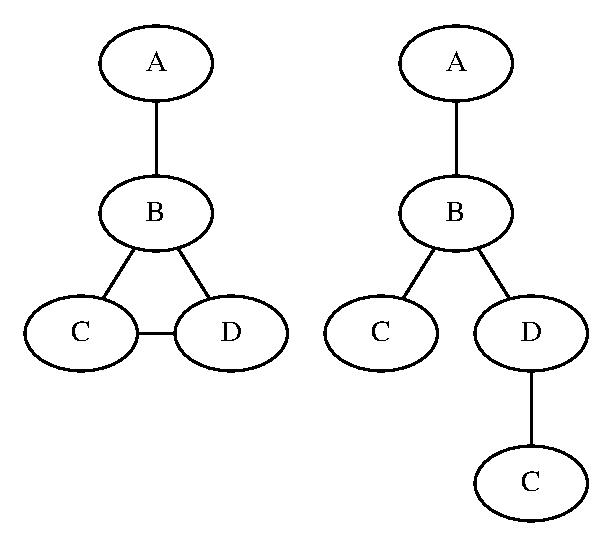
\includegraphics[scale = 0.3]{fig/gab.eps}
\end{center}
\caption{枝刈りに対するfeasible edgeの条件の例}
\label{fig:p}
\end{figure}
\begin{figure}[t]
\begin{center}
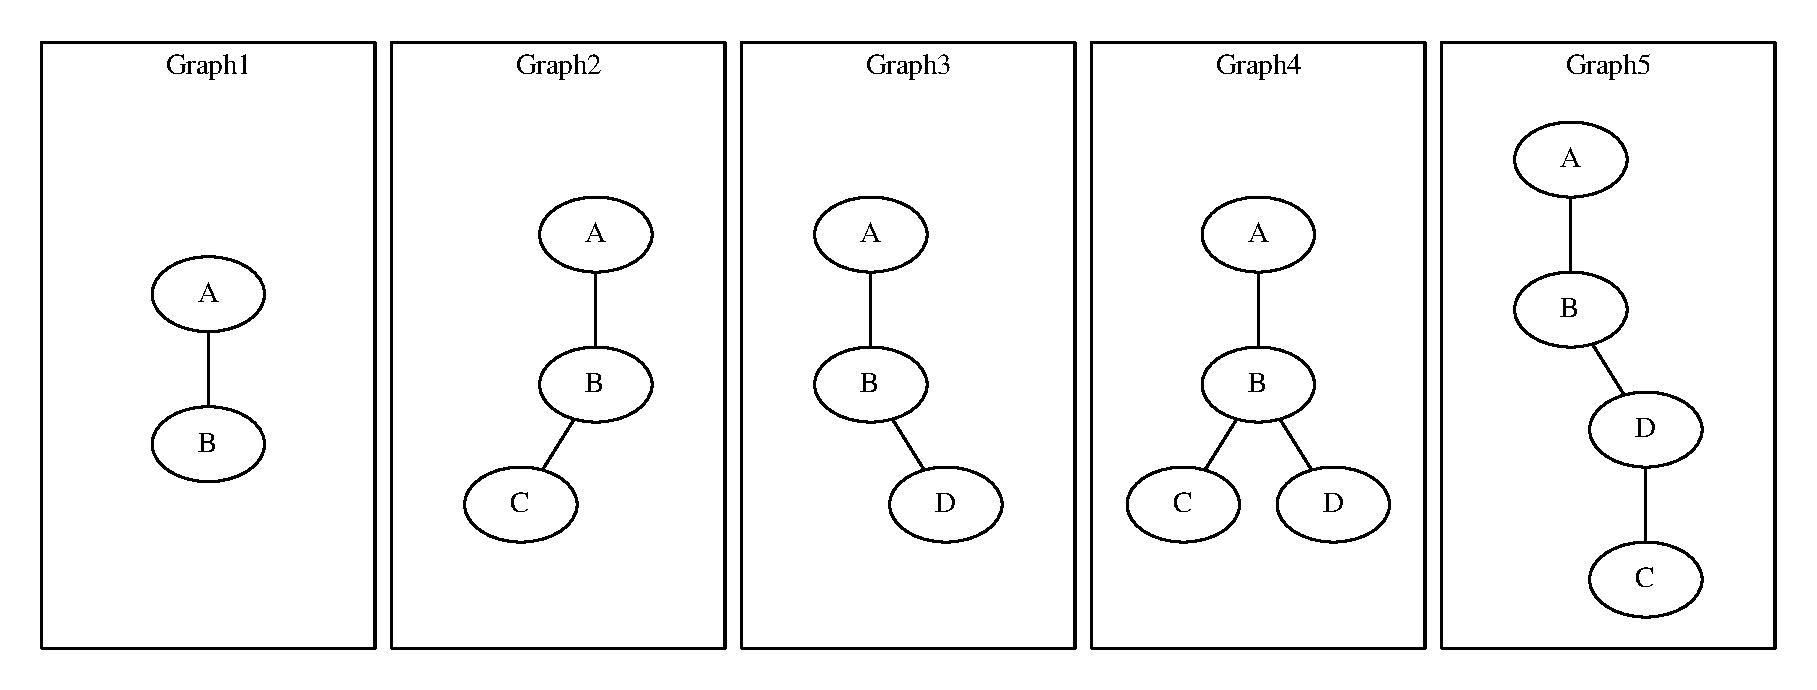
\includegraphics[scale = 0.27]{fig/gabg.eps}
\end{center}
\caption{図\ref{fig:p}のデータベースに対し,minsup=1として頻出部分グラフマイニングをした際の出力グラフ例}
\label{fig:pg}
\end{figure}

必要なパターンを刈ってしまう例を示す.
図\ref{fig:p}の2つのグラフデータベースに対してminsup=1として
頻出部分グラフマイニングをした際の飽和パターン集合を考える.
すると図\ref{fig:pg}のようなパターン例が出現する.
ここでGraph1とGraph2はOMであるために,Graph1の子ノードGraph3は
Graph2の子ノードGraph4があるために飽和パターンではなくなる.それ故に,
Graph1とGraph2がOMであるという条件から
Graph1の他の子ノード(今回はGraph3)が枝刈りができるはずである.しかし,
実際にGraph3を枝刈りすることで,
Graph5のような出現が必要なパターンも同時に枝刈りをしてしまっている.

この問題に対し,Takigawaらは次のような条件と枝刈りを提案した.
\begin{Definition}[Feasible edge]
1つの辺$e$を加えた際,枝刈りが実行可能である場合は$e$が以下のいずれかを満たすときである.
\begin{enumerate}
\renewcommand{\labelenumi}{(\roman{enumi})}
  \item $eが\mathrm{backward\ edge}である.$
  \item $探索している部分グラフが木構造でありかつグラフデータベース中のeがすべてブリッジになっている.$
\end{enumerate}
\end{Definition}
\begin{Theorem}[Right-blanket pruning]
あるグラフ$G$が与えられた時,$G'=G+e\in B_R(G)$が$G$とOMであり,かつ$e$がfeasible edge
であるならば探索木において$G+e',e\neq e'$とその子孫すべてを枝刈りすることができる.
\end{Theorem}
\begin{Theorem}[Left-blanket pruning]
あるグラフ$G$が与えられた時,$G'=G+e\in B_L(G)$が$G$とOMであり,かつ$e$がfeasible edge
であるならば探索木において$G$とその子孫すべてを枝刈りすることができる.
\end{Theorem}


\section{Wildcard許容版$\delta$-tolerance closed frequent subgraphs}

本節では,wildcard許容版$\delta$-tolerance closed frequent subgraphsを求めるアルゴリズムを設計する.それに当たって,まず,wildcardを含めた飽和と極大について新しく定義を追加する.

\subsection{Wildcardを含むパターンに対する飽和集合・極大集合}

\begin{Definition}[Wildcard graphを含むグラフ集合の飽和集合・極大集合]
wildcard graphを含むグラフ集合の飽和集合・極大集合とは,
wildcardを通常のラベルと見なして求めた飽和集合・極大集合から,
wildcardが1つの文字のみにマッチするwildcard graphを除いた集合とする.

%wildcard許容版頻出部分グラフマイニングにおける飽和集合,極大集合では,
%wildcardを他のラベルと同じように1つのラベルとして扱い,
%頻出部分グラフマイニングにおける飽和集合,極大集合と同様に求め,
%さらに,wildcardが複数のラベルを許容しないものを
%必要パターンでないとし,除いたパターン集合である.
\end{Definition}
\begin{figure}[t]
\begin{center}
\includegraphics[scale = 0.28]{fig/wildprun.eps}
\end{center}
\caption{Wildcard pruningと枝刈りをしてはいけない例を示すためのデータベース}
\label{fig:wild}
\end{figure}
\begin{figure}[t]
\begin{center}
\includegraphics[scale = 0.28]{fig/wip-true.eps}
\end{center}
\caption{Wildcardが1種類のラベルのみを許容しているパターン例}
\label{fig:wipt}
\end{figure}

この定義は,wildcard graphにおいて,wildcardが表すラベルがすべて同じで1種類のみである時,
これをwildcardを対応するラベルで置き換えた同一のパターンが存在し,supportが同じであるため
冗長な情報であるとしたものである.
これを図\ref{fig:wild}のデータベースを用いて説明する.
データベースにおいてmisup=2でwildcardを1つ許容した頻出部分グラフマイニング
を行うと,合計24個の部分グラフが出力される.
図\ref{fig:wipt}に示したグラフは頻出なものの中で,
wildcardが1種類のラベルのみを許容しているパターンの例である.
ここに示したグラフ中のwildcardは,
図\ref{fig:wild}のデータベースよりそれぞれ1種類の
ラベルのみにマッチする.したがって,定義5.3より図\ref{fig:wipt}の例のようなグラフは飽和集合・極大集合に含まれない.このようなグラフの除外は,
次の節の更なる枝刈りによって効率化が可能である.

\subsection{Wildcard pruning}
\label{wildprun}
\begin{Lemma}[Wildcard pruning]
あるwildcard graph $G$において,含まれるwildcardが1種類のラベルしか保持しない場合,$G$と以下の子ノードを枝刈りすることができる.
\end{Lemma}

\begin{Proof}
あるwildcard許容グラフ$G$において,含まれるwildcardが1種類のラベルしか持たない時,
そのwildcardを許容しているラベルで置き換えたグラフ$G'$を見た場合,
$GとG'$はデータベース中において指すものが同じなので,OMであり,そのsupportも等しい.
よってGは出力をしなくてよい.また,GのDFSコードの子を考えた時,
そのwildcard graph $G+e$において含まれるwildcardがもつラベルは同様の1種類のラベルのみである.
そのため,$G$と以下すべての子ノードを枝刈りすることができる.\qed
\end{Proof}

\subsection{提案アルゴリズム}
また,wildcard-edge extensionを探索する際にwildcard edgeはextended edgeと同様に扱ってはならない.
その例を図\ref{fig:wild}のデータベースを用いて示す.
まず,このデータベースにおいてminsup=2としてwildcardを1つ許容した頻出飽和部分グラフが
図\ref{fig:wipc}のグラフである.また,この探索を行ったとき,
1-edgeグラフ A-Bから始まる探索木(DFSコード木)が図\ref{fig:ned}である.
この探索木を見ると,A-Bに対してA-B-CがOMであり,かつfeasibleである.
そのため,Right-blanket pruningが適応でき,A-B-Dとそのすべての子ノード
が枝刈りされる.しかし,A-B-$\ast$($\ast$:wildcard)のノードは枝刈りすることができない.
仮に,A-B-$\ast$を枝刈りしてしまうと,図\ref{fig:wipc}に含まれるA-B-$\ast$-Eが出力されない.
これは,A-B-$\ast$のグラフ中のwildcardが許容するラベルが2種類以上あるためである.
つまり$\delta$-tolerance closed frequent subgraphsの枝刈りにおいて,
探索を打ち切ることができるのは通常のextended edgeであって,wildcard edgeを同時に枝刈りすることはできない.
これは,追加した辺に関してOMかつfeasibleであるときに通常のextended edgeと同様にwildcard edgeを枝刈りをしてしまうと,
以上のようなパターンを探索せず,見逃してしまうためである.

\begin{figure}[t]
\begin{center}
\includegraphics[scale = 0.3]{fig/wip-clo.eps}
\end{center}
\caption{minsup=2におけるwildcard 1つ許容した頻出飽和部分グラフ}
\label{fig:wipc}
\end{figure}
\begin{figure}[t]
\begin{center}
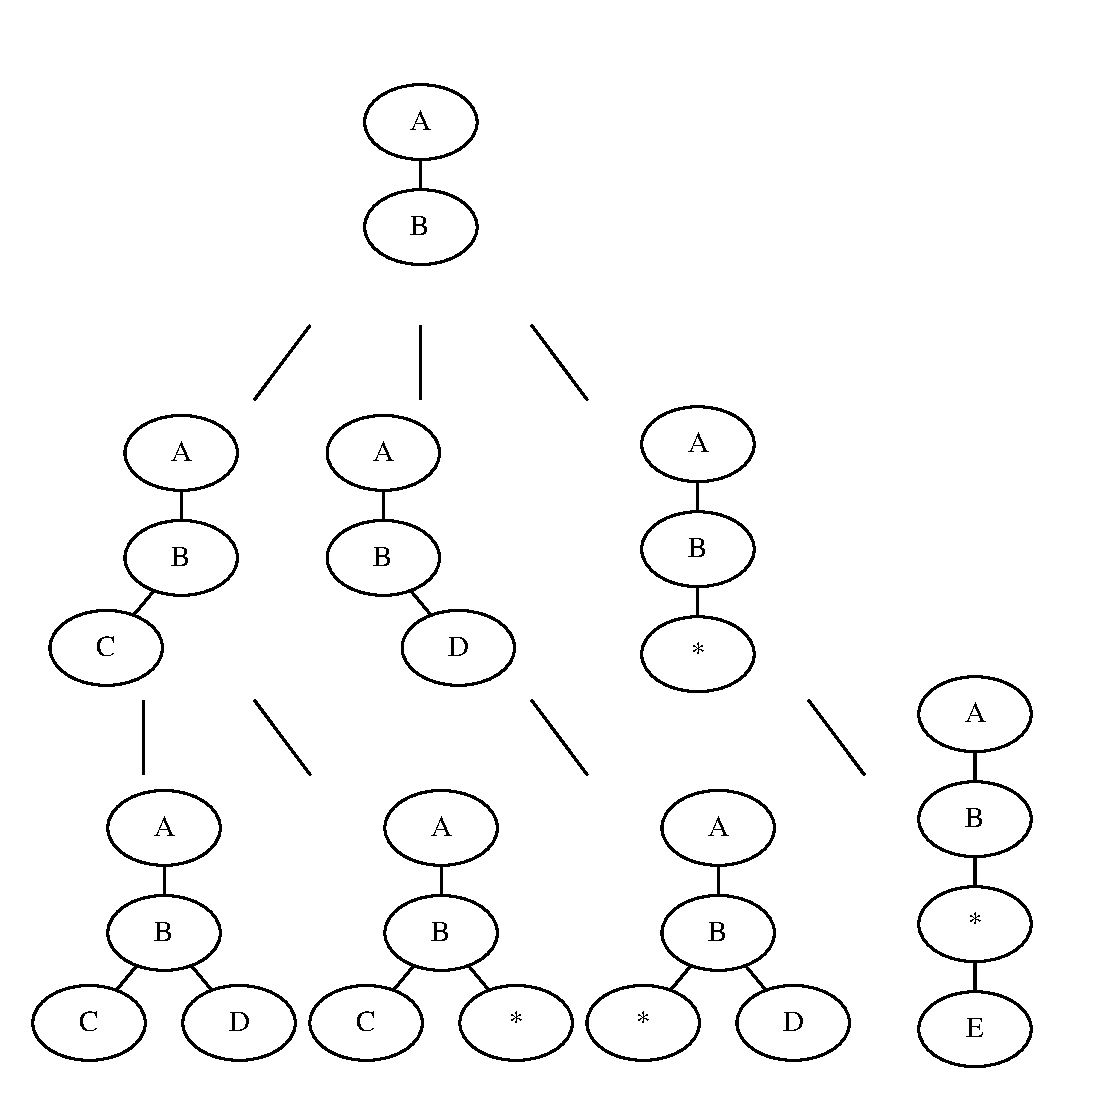
\includegraphics[scale = 0.35]{fig/tree.eps}
\end{center}
\caption{minsup=2におけるwildcard 1つ許容した頻出部分グラフマイニングの探索木(DFSコード木)の一部}
\label{fig:ned}
\end{figure}

これらの条件を考慮することで,wildcard許容版
$\delta$-tolerance closed frequent subgraphsにおいて,
条件を満たすものすべてを全列挙することが可能である.
このアルゴリズムはTakigawaらの$\delta$-tolerance closed frequent subgraphsを拡張した.
Algorithm~\ref{alg2},\ref{pro2},\ref{pro3}に擬似コードを示す.

\begin{algorithm} [t]
\caption{wildcard許容版$\delta$-tolerance closed frequent subgraphs algorithm}         
\label{alg2}                          
\begin{algorithmic} [1] 
\REQUIRE GraphDatabase$\ \mathbb{GS},\mathrm{minsup},\ \delta,\mathrm{wildcard}許容数W$
\ENSURE wildcard$を許容したすべての\delta$-tolerance closed subgraphs
\STATE $\mathbb{GS}内の頂点と辺を出現頻度順にソート$
\STATE $頻出でない頂点と辺を削除$
\STATE $残った頂点と辺を出現頻度の降順にラベル付け$
\STATE $\mathbb{S}^1\leftarrow\mathbb{GS}内のすべての頻出$1-edgeグラフ
\STATE $\mathbb{S}^1_W\leftarrow\mathbb{GS}内のすべての頻出$1-edge\ wildcard graph
\FORALL {$グラフG\in\mathbb{S}^1,\mathbb{S}^1_W$ in DFS辞書順}
\IF {$G$ is wildcard graph}
\STATE $\mathrm{SubgraphMining}(\mathbb{GS},G,W-1)$
\ELSIF {$G$ is not wildcard graph}
\STATE $\mathrm{SubgraphMining}(\mathbb{GS},G,W)$
\ENDIF
\ENDFOR
\end{algorithmic}
\end{algorithm}
\begin{algorithm}[t]
\caption{$\mathrm{SubgraphMining}(\mathbb{GS},G,W)$}         
\label{pro2}                          
\begin{algorithmic} [1] 
\STATE $s:G$のDFSコード
\IF {$G$ is wildcard graph \AND$Gのもつ$wildcardがすべて1種類のラベルを指す}
\STATE return
\ENDIF
\IF {support($G$) $\geq $ minsup}
\STATE return
\ENDIF
\IF {s $\neq$ min(code($G$))}
\STATE return
\ENDIF
\IF {LeftPruning($G$,$\mathbb{GS}$,$W$)}
\STATE $\mathrm{WildcardEdgeExtension}(\mathbb{GS},G,W)$
\STATE return
\ENDIF
\IF {IsDTOLCLOSED($G$,$\mathbb{GS}$,$W$)}
\STATE $現在のパターンを出力$
\ENDIF
\FORALL {$e\in B_R(G)$ in DFS辞書順}
\STATE $\mathrm{SubgraphMining}(\mathbb{GS},G+e,W)$
\IF {$G\longleftrightarrow\hspace{-1.75em}\raisebox{.9ex}{\tiny OM}\ \ G+e$ \AND$e$ is feasible}
\STATE $\mathrm{WildcardEdgeExtension}(\mathbb{GS},G,W)$
\STATE return
\ENDIF
\ENDFOR
\STATE $\mathrm{WildcardEdgeExtension}(\mathbb{GS},G,W)$
\end{algorithmic}
\end{algorithm}

\begin{algorithm}[t] 
\caption{$\mathrm{WildcardEdgeExtension}(\mathbb{GS},G,W)$}         
\label{pro3}                          
\begin{algorithmic} [1] 
\IF {$W=0$}
\STATE return
\ENDIF
\FORALL {$e\in B_R^W(G)$ in DFS辞書順}
\STATE $\mathrm{SubgraphMining}(\mathbb{GS},G+e,W)$
\ENDFOR
\end{algorithmic}
\end{algorithm}



\if0
\begin{algorithm}
\floatname{algorithm}{Procedure}  
\caption{$LeftPruning(G,\mathbb{GS},W)$}         
\label{pro4}                          
\begin{algorithmic} [1] 
\STATE $X\leftarrow\emptyset;i\leftarrow1;$
\FORALL {$\mathbb{GS}に出現するG$}
\STATE $Y_i\leftarrow\emptyset;$
\FORALL {$G+e\in B_L(G) in DFS辞書順$}
\IF {$e=\mathrm{feasible\ edge}$}\STATE $Y_i\leftarrow\{G+e\} \cap Y_i$\ENDIF
\ENDFOR
\IF {$W>0$}
\FORALL {$G+e\in B^W_L(G) in DFS辞書順$}
\IF {$e=\mathrm{feasible\ edge}$}
\STATE $Y_i\leftarrow\{G+e\} \cap Y_i$
\ENDIF
\ENDFOR
\ENDIF
\IF {$i=1$}
\STATE $X\leftarrow Y_i$
\ELSE
\STATE $X\leftarrow X\cap Y_i$
\IF {$X = \emptyset$}\RETURN \FALSE\ENDIF
\ENDIF
\STATE $i\leftarrow i+1$
\ENDFOR
\RETURN \TRUE 
\end{algorithmic}
\end{figure}

\begin{algorithm}
\floatname{algorithm}{Procedure}  
\caption{$IsDTOLCLOSED(G,\mathbb{GS},W)$}         
\label{pro5}                          
\begin{algorithmic} [1] 
\STATE $X\leftarrow\emptyset;i\leftarrow1;$
\STATE $\theta \leftarrow max((1-\delta)\cdot support(G),minsup)$
\STATE $m\leftarrow 0;i\leftarrow1;$
\FOR {$\mathbb{GS}のうちGを含むGS_i$}
\IF{$W=0$} \STATE{$Y_i\leftarrow \{G+e\in B(G)\mid G+e in GS_i\}$} 
\ELSE \STATE{$Y_i\leftarrow \{G+e\in B(G),B^W(G)\mid G+e in GS_i\}$} \ENDIF
\STATE $X_i\leftarrow X \cup Y_i$
\FOR {$G'\in X$}
\STATE $sup_i\leftarrow support(G' \mid \{ GS_1,\dots,GS_i\})$ 
\IF{$sup_i < i-support(G)+\theta$}  \STATE{$X\leftarrow X\setminus \{G'\}$} \ENDIF
\IF{$sup_i>m$}  \STATE{$m\leftarrow sup_i$} \ENDIF
\ENDFOR
\IF{$X=\emptyset$\AND$i>support(G)-\theta$} \RETURN \TRUE  \ENDIF
\IF{$X\neq\emptyset$\AND$m\geq \theta$} \RETURN \FALSE  \ENDIF
\STATE $i\leftarrow i+1$
\ENDFOR
\end{algorithmic}
\end{algorithm}
\fi


まずAlgorithm~\ref{alg2}において,探索木のはじめのノードとなる1-edgeグラフにおいて考えうるすべてのwildcardをもつグラフを追加する.

次にAlgorithm~\ref{pro2}の$\mathrm{SubgraphMining}(\mathbb{GS},G,W)$では,現在のパターンについて$\delta$-tolerance closedであるか
を探索し,子ノードとして考えうるすべてのパターンを再帰的に呼び出すものである.
Algorithm~\ref{pro2}の2行目で現在のパターンがwildcardを含むグラフで
あるとき,そのwildcardの現れる場所全てにおいて同じラベルを表す,つまりすべてのwildcardが1種類のラベルを表すならば,
wildcard pruningを満たしそのパターンとその子ノードすべては必要なパターンではないので枝刈りをする.
この枝刈りの判定するために
WildcardEdgeExtensionの際に調べたwildcardをその後の子ノードで保持しておく必要があるため,
wildcard graphはwildcardを持つ場所とそのラベルをデータ構造上にもつ.
また,$\delta$-tolerance closed frequent subgraphsと同様に,
Left-blanket pruningにより枝刈りができるかを探索し,$\delta$-tolerance closedであるかどうかを調べ,
Right-blanket pruningによる枝刈りの探索をする.
しかし,前に述べたようにLeft-blanket pruningとRight-blanket pruningによる枝刈りの条件を満たしていたとしてもwildcard edgeの探索はしなければならない.
そのため,Algorithm~\ref{pro2}の3箇所にAlgorithm~\ref{pro3}のWildcardEdgeExtension$(\mathbb{GS},G,W)$を入れる必要がある.
Algorithm~\ref{pro3}は擬似コードが複雑にならないように分けたものである.

%procedure\ref{pro4}の
$\mathrm{LeftPruning}(G,\mathbb{GS},W)$,
%procedure\ref{pro5}の
$\mathrm{IsDTOLCLOSED}(G,\mathbb{GS},W)$は
$\delta$-tolerance closed frequent subgraphsにおける定義\cite{deltol}に,
現在のパターンに更にwildcardの拡張ができる場合,
通常のものと同様にwildcard edgeも調べるように拡張したものであるため,ここでは省略する.


\newpage
%exp.tex ・・・実験の章(別ファイル)

\chapter{実験と考察}

この章では,これまでに述べたwildcardを許容することで頻出部分グラフマイニング
による出力がどれほど増え,出力時間が長くなるかを実験する.
さらに,提案した飽和・極大パターンにより,どれほど出力が抑えられるか,
出力時間はどのように変化するかを実験,検証する.

また,wildcardを許容した部分グラフパターンがどれほど有用であるかを,
機械学習の特徴として用いることで検証する.

\section{実験環境}
本手法を実装したものの実験環境として,以下を使用した.

\begin{center}
\begin{tabular}{cl}
\hline
CPU& Intel(R) Core(TM) i7-3770K 3.50GHz\\
\hline
メモリ&33GB\\
\hline
OS &Ubuntu 14.04.3 LTS\\
\hline
\end{tabular}
\end{center}

\section{使用したデータベース}
今回,Takigawaら\cite{deltol}によって用いられたMutagとCPDBの2つのデータを使用し,実験を行った.
それぞれのデータベースのグラフ数,平均ノード数,平均エッジ数を表\ref{dataset}に示す.AIDS(CAvsCM)
に関しては,機械学習に対する実験で使用した.
\begin{table}[h]
\caption{使用したデータセット}
\begin{center}
\begin{tabular}{|c|l|l|l|}
\hline
 &グラフ数&平均ノード数&平均エッジ数\\
\hline
Mutag &188&17.9&19.8\\
\hline
CPDB&684&14.1&14.6\\
\hline
AIDS(CAvsCM)&1503&59.0&61.6\\
\hline
\end{tabular}
\end{center}
\label{dataset}
\end{table}
\section{出力数と出力時間に関する実験}
\label{out-exp}

頻出部分グラフマイニングにwildcardを許容した場合の出力数,CPUtimeの比較を行う.
さらに増加した出力数が,wildcard許容版$\delta$-tolerance closed frequent subgraphs algorithmによって抑えられているのか実験した結果を出力数とCPUtimeの観点から検証する.

この実験では頂点のラベルにのみwildcardを許容した.これは使用するデータが化合物データであり,化合物データにおいて辺のラベルは
結合数を指すことが多いため,辺のラベルにwildcardを考える必要はないと判断したためである.
しかし,一般的なグラフデータベースにとって辺のラベルが重要な情報を持つことは少なくないため,
辺のラベルに対してwildcardを許容するべき時もあるが,これは頂点のラベルと同様に拡張可能である.


図\ref{cpdb}に実験結果を示す.
図\ref{cpdb}左がMutag,図\ref{cpdb}右がCPDBの実験結果で,それぞれ上図が出力数,
中央図がCPUtime,下図が1出力あたりのCPUtimeの実験結果を表している.
図中においてgSpanは通常の頻出部分グラフマイニング,
gSpan with wildcardはwildcardを1つ許容した頻出部分グラフマイニング,
closed with wildcard,maximal with wildcardはそれぞれ
wildcardを1つ許容した頻出部分グラフマイニングに対する
頻出飽和パターン集合,頻出極大パターン集合の結果である.

\subsection{考察}

Mutagの実験結果では,図\ref{cpdb}左において,gSpanとgSpan with wildcardを比較すると,
misupをさげるとどちらも指数的に出力が伸びているのに対し,
minsupを固定して比較すると,出力数はほぼ定数倍であることがわかる.
CPDBの結果でも同様のことが言え,
これはすべての頻出部分グラフのすべての頂点ラベルに対して
wildcardを許容した場合を考えることができるためであり,
通常の頻出部分グラフに対して出力部分グラフの平均ノード数倍の出力が得られるものと考えられる.
またCPUtimeにおいて,gSpanとgSpan with wildcardを比較すると,
図\ref{cpdb}の左右の中央図より,
こちらもほぼ定数倍で増えていることがわかる.
これは図\ref{cpdb}の下図より見て取れるように
,gSpanとgSpan with wildcardの1つあたりのCPUtimeはほぼ同じであるためである.

実験結果より,頻出部分グラフマイニングではminsupを下げると指数倍以上に出力が増える.
さらに,wildcardを許容することでほぼ定数倍ではあるが出力数が増え,扱いがより困難になると考えられる.
そこで飽和・極大パターン集合による集合要約の効果を検証する.

まずはMutagとCPDBのデータの違いによる差をみると,
MutagはCPDBに比べデータ数は少ないが平均のグラフサイズが大きく,
頻出部分グラフマイニングから見られるように出力数が多いことから
似たグラフが多いことがみてとれる.
それに比べCPDBではグラフデータベースが疎であるためか,
頻出部分グラフがMutagに比べて少ない.

図\ref{cpdb}の左右の上図,中央図より,
飽和・極大パターン集合を求めると通常の部分グラフパターンより時間がかかるが,
出力はかなり抑えられていることが,実験結果よりわかる.
さらに$\delta$の指標により飽和と極大の集合間の出力を
自由に決めることができる.今回の実験では,$\delta$を変えた実験は追加していない
が,原理上,飽和と極大の間になる.

図\ref{cpdb}の左右の下図より,
MutagとCPDBの両者に見られるようにwildcardを許容した頻出部分グラフの
飽和・極大パターン集合は頻出部分グラフの増加傾向ほど
増えないためminsupをさげると通常の頻出部分グラフ数ほどの出力まで抑えられている.
さらにMutagはCPDBに比べ似たグラフが多いためその傾向が顕著にあらわれている.
図\ref{cpdb}右の中央図からわかるように,
CPUtimeでは出力数が増えた場合,枝刈りが有効で,
wildcardを許容した頻出部分グラフマイニングに対して
飽和・極大パターン集合のほうが時間がかからなくなることもある.

\begin{figure}[H]
\begin{tabular}{cc}
      Mutag &  CPDB \\ 
    \begin{minipage}{80mm}
      \centering
      \scalebox{1.1}{\includegraphics{fig/mutag_out.eps}}
    \end{minipage} &
    \begin{minipage}{80mm}
      \centering
      \scalebox{1.1}{\includegraphics{fig/cpdb_out.eps}}
    \end{minipage} \\ 
    \begin{minipage}{80mm}
      \centering
      \scalebox{1.1}{\includegraphics{fig/mutag_time.eps}}
    \end{minipage} &
    \begin{minipage}{80mm}
      \centering
      \scalebox{1.1}{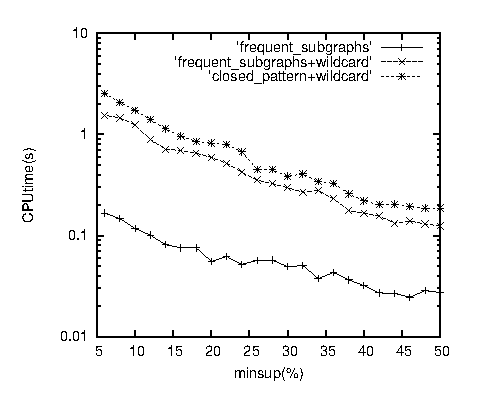
\includegraphics{fig/cpdb_time.eps}}
    \end{minipage} \\
    \begin{minipage}{80mm}
      \centering
      \scalebox{1.1}{\includegraphics{fig/per_mutag.eps}}
    \end{minipage} &
    \begin{minipage}{80mm}
      \centering
      \scalebox{1.1}{\includegraphics{fig/per_cpdb.eps}}
    \end{minipage} \\

  \end{tabular}
\caption{Mutag(左)CPDB(右)の実験結果:上から順に出力数,CPUtime,1出力あたりのCPUtime}
\label{cpdb}
\end{figure}

%\newpage
\section{機械学習に対する応用実験}
本節では,実験に用いたデータセットに対して,マイニングにより出力された
パターンの0,1ベクトルを2クラス分類の機械学習の特徴ベクトルとして
機械学習を行う.さらにその精度を比べることで,wildcardを許容した
パターンがどれほど有効であるかを検証する.機械学習として
用いた手法はSVM,Random Forestである.%どこまで説明する???

SVM(サポートベクターマシン) は2クラスの分類問題を解くための学習器である.
SVM は線形の識別器で,カーネルを組み合わせることによって非線形に拡張することができる.
これまで,文字認識や画像認識などの分野で利用され,高い識別能力を示している.

Random Forestは決定木を弱学習器とする集団学習アルゴリズムで,
ランダムサンプリングされたトレーニングデータによって学習した多数の決定木を使用し
分類器を形成する.Random Forestは説明変数(ここでは特徴パターン)が多数であっても
うまく動き,学習・評価が高速である.

\subsection{実験準備}

今回行う,2クラス分類では,次のようなデータセット
$D=\{(\vector{x}_i,y_i)\ |\ \vector{x}_i\in \mathbb{R}^p,y_i\in \{-1,1\}\}$
を与える.ここで,pは次元数(特徴パターン数)を指す.

この特徴ベクトル$\vector{x}$を
%本実験において比較する特徴は,
通常の頻出部分グラフ,wildcard許容頻出部分グラフ
それぞれに対して求め,比較を行う.
実験1として,膨大なパターン数をminsupで枝刈りすることで求める.
これを\ref{subsec:exp1}で,実験結果を示し,考察を行う.
\if0
通常,minsupで枝刈りをする方法は,データベース中の
すべてのグラフをうまく説明できないため,
十分にminsupを下げなければ
機械学習の特徴としてはあまり精度がでない.
minsupでは枝刈りをせず,部分グラフのエッジ数で決まるパターンの長さ
(以下,maxpat)で枝刈りしたパターンを使用したほうがいい例もあると
提案されている.%GFの引用
そこで,実験2として,本研究では,maxpatで枝刈りをする方法について
,wildcardを許容したパターンが有効であるか実験を行う.
これを\ref{subsec:exp2}で示し,考察を行う.
\fi
wildcard許容に対して,出力増加の問題があることを\ref{out-exp}
で示した.通常の頻出部分グラフに対する飽和・極大パターン
による機械学習は,本研究においては問題視しない.
しかし,wildcardを含むパターンに対して,
冗長なパターンを削除することは,大変重要な問題である.
本論文において,wildcardに対する飽和・極大に対して,
すでに存在しているパターンと冗長なものを削減する方法
を\ref{wildprun}で提案した.実験2として,頻出部分グラフマイニングに対して
wildcardを許容したパターンとそれに対してwildcard pruningによる枝刈りのみを
行ったパターンに対して,出力と出力時間の比較を行う.
さらに,これに対して機械学習を行った精度の比較を行う.
これを\ref{subsec:exp3}で示し,考察を行う.

本研究では,定めた手法に対して10-分割交差検証
を行い,精度を比較する.
まず,与えられたデータセット$D$に対して10通りの分割を
行いトレーニングデータとテストデータに分ける.
そして,それぞれのトレーニングデータに対して,
通常の頻出部分グラフ,wildcard許容頻出部分グラフを求め,
グラフデータベース中のそれぞれのグラフにおいて,
求めた特徴を持つか持たないかを表す0,1ベクトルを
特徴ベクトル$\vector{x}$とする.以上を入力とし,
それぞれのデータセットに対して分類器を学習し,
そのテストデータに対する正解率の平均値をその手法の精度としている.

使用したSVMのパラメータでは,
$C=1, 10,100,1000,10000, kernel=linearと
C=1,10,100,1000,gamma=0.001,0.0001,kernel=rbf$
でグリッドサーチを行っており,時間の都合上
AIDSのデータでは決め打ちでC=1,gamma=0.001,kernel=rbfで実験を行った.
%SVMのパラメータ決めの話をするか
%AIDSのデータでは決め打ちでC=1,gamma=0.001,kernel='rbf'


\if0
頻出飽和部分グラフについては,基本的に情報が失われておらず,
頻出極大部分グラフにおいては情報を失っているため,
機械学習に対しては精度が期待できない.そのため,
本論文において,頻出飽和・極大部分グラフパターンに対しては,
実験を行っていない.

さらに,通常の頻出部分グラフ,wildcard許容頻出部分グラフ,
wildcard pruningによる枝刈りのみを行ったwildcard許容頻出部分グラフ,
それぞれに対して,minsupを変えることができ,精度が変わるため
minsupを変えた実験を行う.

さらに,minsupを1(最低1つ以上に現れる部分グラフ)
のうち,パターンの長さの最大値(maxpat)を決め枝刈りをする手法が存在し,%引用せねば
これに対しても実験を行う.yo
\fi
\subsection{実験1:結果と考察}
\label{subsec:exp1}%この章のLabel

図\ref{ml_minsup}にwildcard許容に対するminsupを変動させた時の実験結果を示す.
上段がMutag,中央段がCPDB,下段がAIDS(CAvsCM)に対する実験結果であり,
それぞれ左にSVM,右にRandom Forestの実験結果である.

図\ref{ml_minsup}に示した実験結果のうちMutag,AIDS(CAvsCM)は
minsupを下げられる範囲のもので,これ以上さげると,使用した実行環境では実行できない.

図\ref{ml_minsup}上段のMutagでは,
SVMに対してminsup35-50では良い結果が出ている部分があり,
Random Forestを見ると精度に差がない.
Mutagデータセットに関して,使用した実験環境で実行できる範囲で
一番よい結果が得られているのは,wildcardを1つ許容した時で,
minsup=42の時である.Random Forestでは,精度の最大値ではほぼ変わらないと言える.

図\ref{ml_minsup}中央段のCPDBでは,
いずれの手法も,minsupが20以上で良い結果が得られている.
minsupを十分に下げるとあまり精度に差がないが,
通常の頻出部分グラフパターンによる結果と同等か,
それ以上の結果が出ている.
さらにminsup=44の時の結果がよく出ており,
minsupを下げずに良い結果を得られていると言える.

図\ref{ml_minsup}中央段のAIDS(CAvsCM)では,
wildcardを許容することにより求められる範囲が狭くなる上,
精度が落ちていることがわかる.通常の頻出部分グラフパターン
に対して見ると,minsupを下げることで精度が落ちているため,
この2値分類問題に対しては頻出部分グラフパターン自体が
あまり良い結果につながらない可能性がある.

以上の実験結果より,
wildcardが有効であるデータベースとそうでないデータベースが
存在するが,minsupを下げると精度が上がるような問題に対して,
wildcardを許容することで,精度が下がることはなく,
状況により精度が上がる.
これは,データベースに対して,それらをうまく表現するような
特徴としての候補を得ることができるためだと考えられる.
つまり,頻出パターンによる機械学習の傾向が一般的な
(MutagやCPDBのようにminsupを下げると基本的に精度が良くなる)
場合には,wildcardを入れるのは有効であると言えるような実験結果となった.

\begin{figure}[H]
  \begin{tabular}{cc} % l:左寄せ,c:中央揃え r:右寄せ 
      Mutag-SVM &  Mutag-RF \\ 
    \begin{minipage}{80mm}
      \centering
      \scalebox{1.1}{\includegraphics{fig/mutag_svm.eps}}
    \end{minipage} &
    \begin{minipage}{80mm}
      \centering
      \scalebox{1.1}{\includegraphics{fig/mutag_rf.eps}}
    \end{minipage} \\ 
      CPDB-SVM &  CPDB-RF \\ 
    \begin{minipage}{80mm}
      \centering
      \scalebox{1.1}{\includegraphics{fig/cpdb_svm.eps}}
    \end{minipage} &
    \begin{minipage}{80mm}
      \centering
      \scalebox{1.1}{\includegraphics{fig/cpdb_rf.eps}}
    \end{minipage} \\
      AIDS(CAvsCM)-SVM &  AIDS(CAvsCM)-RF \\ 
    \begin{minipage}{80mm}
      \centering
      \scalebox{1.1}{\includegraphics{fig/cacm_svm.eps}}
    \end{minipage} &
    \begin{minipage}{80mm}
      \centering
      \scalebox{1.1}{\includegraphics{fig/cacm_rf.eps}}
    \end{minipage} \\

  \end{tabular}
  \caption{Mutag(上)CPDB(中央)AIDS(CAvsCM)(下)のminsupの変化と正解率の実験結果:左から順にSVM,Random Forest}
  \label{ml_minsup} % \ref{ラベル名}で表番号を参照
\end{figure}

\if0
\subsection{実験2:結果と考察}
\label{subsec:exp2}%この章のLabel

図\ref{ml_maxpat}にwildcard許容に対するmaxpatを変動させた時の実験結果を示す.
上段がMutag,下段がCPDBに対する実験結果であり,
それぞれ左にSVM,右にRandom Forestの実験結果である.

以下,考察

\begin{figure}[H]
  \begin{tabular}{cc} % l:左寄せ,c:中央揃え r:右寄せ 
      Mutag-SVM &  Mutag-RF \\ 
    \begin{minipage}{80mm}
      \centering
      \scalebox{1.1}{\includegraphics{fig/mutag_svm_maxpat.eps}}
    \end{minipage} &
    \begin{minipage}{80mm}
      \centering
      \scalebox{1.1}{\includegraphics{fig/mutag_rf_maxpat.eps}}
    \end{minipage} \\ 
      CPDB-SVM &  CPDB-RF \\ 
    \begin{minipage}{80mm}
      \centering
      \scalebox{1.1}{\includegraphics{fig/cpdb_svm_maxpat.eps}}
    \end{minipage} &
    \begin{minipage}{80mm}
      \centering
      \scalebox{1.1}{\includegraphics{fig/cpdb_rf_maxpat.eps}}
    \end{minipage} \\

  \end{tabular}
  \caption{Mutag(上)CPDB(下)のmaxpatの変化と正解率の実験結果:左から順にSVM,Random Forest}
  \label{ml_maxpat} % \ref{ラベル名}で表番号を参照
\end{figure}

\fi

\subsection{実験2:結果と考察}
\label{subsec:exp3}%この章のLabel

図\ref{wildpruning-out}にwildcard許容に対してwildcard pruningによる枝刈りによる出力と出力時間の実験結果を示す.
それぞれ左にMutag,右にCPDBの実験結果で,上段が出力数,下段が出力時間に対する実験結果である.

図\ref{ml_wildpruning_mutag},図\ref{ml_wildpruning_cpdb}にwildcard許容に対して
wildcard pruningによる枝刈りによる特徴削減の実験結果を示す.
図\ref{ml_wildpruning_mutag}がMutag,図\ref{ml_wildpruning_cpdb}がCPDBに対する実験結果である.
それぞれ左にSVM,右にRandom Forestの実験結果である.

図\ref{wildpruning-out}左上より,
Mutagではwildcard pruningによる枝刈りによりパターン数が抑えられており,
wildcard許容頻出部分グラフに対して余計な処理を行った時間に対して,
minsupを下げた場合に出力時間が抑えられていることが図\ref{wildpruning-out}左下
からわかる.

しかし,図\ref{wildpruning-out}右側より,
CPDBではほぼ出力数は変化していないため,出力時間では
元より少し時間がかかる結果となった.

一方で,機械学習に対する変化であるが,
精度に対して,変動こそあるものの一方的に悪くなったり
良くなったりしているわけではなく,誤差の範囲と言えるだろう.

また,Mutagに関しては,図\ref{ml_wildpruning_mutag}より,出力が抑えられるため,
元よりminsupを下げたところまで求めることができ,良い結果が出ている部分もある.


\begin{figure}[htb]
  \begin{tabular}{cc} % l:左寄せ,c:中央揃え r:右寄せ 
      Mutag-SVM &  CPDB \\ 
    \begin{minipage}{80mm}
      \centering
      \scalebox{1.1}{\includegraphics{fig/wildcard_mutag_out.eps}}
    \end{minipage} &
    \begin{minipage}{80mm}
      \centering
      \scalebox{1.1}{\includegraphics{fig/wildcard_cpdb_out.eps}}
    \end{minipage} \\ 
    \begin{minipage}{80mm}
      \centering
      \scalebox{1.1}{\includegraphics{fig/wildcard_mutag_time.eps}}
    \end{minipage} &
    \begin{minipage}{80mm}
      \centering
      \scalebox{1.1}{\includegraphics{fig/wildcard_cpdb_time.eps}}
    \end{minipage} 
  \end{tabular}
  \caption{Mutag(左)CPDB(右)のwildcard pruningによる出力と出力時間の実験結果:上から順に出力数,出力時間}
  \label{wildpruning-out} % \ref{ラベル名}で表番号を参照
\end{figure}


\begin{figure}[htb]
  \begin{tabular}{cc} % l:左寄せ,c:中央揃え r:右寄せ 
      wildcard1-SVM &  wildcard1-RF \\ 
    \begin{minipage}{80mm}
      \centering
      \scalebox{1.1}{\includegraphics{fig/mutag_svm_wildcard1_pruning.eps}}
    \end{minipage} &
    \begin{minipage}{80mm}
      \centering
      \scalebox{1.1}{\includegraphics{fig/mutag_rf_wildcard1_pruning.eps}}
    \end{minipage} \\ 
      wildcard2-SVM &  wildcard2-RF \\ 
    \begin{minipage}{80mm}
      \centering
      \scalebox{1.1}{\includegraphics{fig/mutag_svm_wildcard2_pruning.eps}}
    \end{minipage} &
    \begin{minipage}{80mm}
      \centering
      \scalebox{1.1}{\includegraphics{fig/mutag_rf_wildcard2_pruning.eps}}
    \end{minipage} \\
  \end{tabular}
  \caption{Mutagのwildcard pruningによる特徴削減の実験結果:左から順にSVM,Random Forest}
  \label{ml_wildpruning_mutag} % \ref{ラベル名}で表番号を参照
\end{figure}

\begin{figure}[htb]
  \begin{tabular}{cc} % l:左寄せ,c:中央揃え r:右寄せ 
      wildcard1-SVM &  wildcard1-RF \\ 
    \begin{minipage}{80mm}
      \centering
      \scalebox{1.1}{\includegraphics{fig/cpdb_svm_wildcard1_pruning.eps}}
    \end{minipage} &
    \begin{minipage}{80mm}
      \centering
      \scalebox{1.1}{\includegraphics{fig/cpdb_rf_wildcard1_pruning.eps}}
    \end{minipage} \\ 
      wildcard2-SVM &  wildcard2-RF \\ 
    \begin{minipage}{80mm}
      \centering
      \scalebox{1.1}{\includegraphics{fig/cpdb_svm_wildcard2_pruning.eps}}
    \end{minipage} &
    \begin{minipage}{80mm}
      \centering
      \scalebox{1.1}{\includegraphics{fig/cpdb_rf_wildcard2_pruning.eps}}
    \end{minipage} \\

  \end{tabular}
  \caption{CPDBのwildcard pruningによる特徴削減の実験結果:左から順にSVM,Random Forest}
  \label{ml_wildpruning_cpdb} % \ref{ラベル名}で表番号を参照
\end{figure}

\newpage
%result.tex ・・・まとめの章(別ファイル)

\chapter{まとめ}
\section{結論}
本研究では,頻出部分グラフマイニングのアルゴリズムであるgSpan,
さらに$\delta$-tolerance closed frequent subgraphs algorithm
を拡張し,wildcardを許容した頻出部分グラフパターンの列挙と
その飽和パターン集合・極大パターン集合を求める手法を提案した.
さらに実験から,wildcardを許容することによる頻出パターン数の増加を示し,
飽和パターン・極大パターンによるパターン集合要約の効果を確かめた.
さらに,wildcardを許容した頻出部分グラフが実際に有用なパターンで
あるかを,機械学習に対する特徴として用いることで効果検証した.
その結果,グラフデータセットによっては効果的な出力があり,
wildcardを許容に対して有効であると言える傾向実験結果を得た.
また,冗長なパターンを削減することで,精度を下げずに,
よりうまく応用できる.
%いい結果と呼べること

\section{今後の展望}
今回検証した実験に対して,さらに実験を行うことで
今回得た結果に対する考察の信憑性を確かめる必要があるだろう.
また,今回は正解率による検証を行ったが,
ここからグラフをよりうまく分類できている特徴を
見ることで,wildcardを許容した部分グラフがどれほど
選ばれているのか調べる必要がある.
さらに,通常,minsupで枝刈りをする方法は,データベース中の
すべてのグラフをうまく説明できないため,
十分にminsupを下げなければ
機械学習の特徴としてはあまり精度がでない.
minsupでは枝刈りをせず,部分グラフのエッジ数で決まるパターンの長さ
で枝刈りをする方法もあり,これに対しても
検証を行ったが,うまく説明できるような結果でなかったため,
さらに実験をし,傾向を確認したい.



\chapter*{謝辞}
\addcontentsline{toc}{chapter}{謝辞}

本研究を進めるに当たり,本研究に関する専門的な知識やアイデア,
研究の方向性,論文の構成から体裁に至るまで,
多大な助言・ご指導をいただきました瀧川一学准教授,
また技術・知識だけでなく,日常の学生生活において
多大なご指導をいただいた湊真一教授に深く感謝いたします.
また,本研究に関して議論を交わし,
多くの助言をいただいたERATO研究員の皆様,研究室の皆様,
研究活動を支えてくださいました家族に深く感謝いたします.
また,本研究に当たって様々な知識・技術に関するご指導をいただいたすべての皆様に
感謝を申し上げます.

\newpage
\if0
\begin{thebibliography}{99}% 文献数が10未満の時 {9}
\bibitem{fssm}
J.Huan,  W.Wang  and  J.Prins," Efficient  mining  of 
frequent  subgraphs  in  the  presence  of  isomorphism," 
ICDM   ’03:   Proceedings   of   the   Third   IEEE 
International Conference on Data Mining, Washington,
DC, USA, IEEE Computer Society, pp. 549--552,2003.   
\bibitem{fsg}
M.Kuramochi  and  G. Karypis, " Frequent  subgraph 
discovery," ICDM ’01: Proceedings of the 2001 IEEE 
International Conference on Data Mining, Washington,
DC,  USA,  IEEE  Computer  Society,  pp.313--320,2001.  

\bibitem{agm1}
A.Inokuchi, T.Washio and H.Motoda, "  An 
apriori-based    algorithm    for    mining    frequent 
substructures    from    graph    data, "   PKDD    ’00: 
Proceedings  of  the  4th  European  Conference  on 
Principles of Data Mining and Knowledge Discovery, 
London,UK,Springer-Verlag, pp.13--23 2000.   
\bibitem{agm2}
A. Inokuchi,  T. Washio  and  H. Motoda, " Complete 
mining  of  frequent  patterns  from  graphs"  Mining 
graph data, Mach. Learn. pp. 321--354,2003. 
\bibitem{acgm}
A. Inokuchi, T. Washio, K. Nishimura and H. Motoda,
"A  Fast  Algorithm  for  Mining  Frequent  Connected 
Subgraphs,"  IBM  Research,  IBM  Research  Report ,2002.   


\bibitem{gSpan}
X. Yan  and  J. Han,"  gspan:  Graph-based  substructure 
pattern  mining,"  ICDM  ’02:  Proceedings  of  the  2002 
IEEE   International   Conference   on   Data   Mining 
,  Washington,  DC,  USA,  IEEE  Computer 
Society, pp. 721--724 ,2002.  
\bibitem{gaston}
S. Nijssen  and  J. N.  Kok,"  A  quickstart  in  frequent 
structure  mining  can  make  a  difference,"  KDD  ’04: 
Proceedings of the tenth ACM SIGKDD international 
conference on Knowledge discovery and data mining, 
New  York,  NY,  USA,  ACM  Press,pp.647--652,2004.  


\bibitem{wildcard}
H. Hofer, C. Borgelt, and M.R. Berthold.," Large scale mining of molecular fragments with wildcards.," In Advances in Intelligent Data Analysis V, pp. 380--389,2003.
\bibitem{ws1}
Xie, F., Wu, X., Hu, X., Gao, J., Guo, D., Fei, Y., and Hua, E.,
"Sequential pattern mining with wildcards.," In Tools with Artificial Intelligence (ICTAI), 2010 22nd IEEE International Conference ,Vol. 1, pp. 241-247,2010.
\bibitem{ws2}
He, Y., Wu, X., Zhu, X., and Arslan, A. N.," Mining frequent patterns with wildcards from biological sequences.,"In Information Reuse and Integration, 2007. IRI 2007. IEEE International Conference ,pp. 329-334,2007.
\bibitem{ws3}
Wu, X., Zhu, X., He, Y., and Arslan, A. N.," PMBC: Pattern mining from biological sequences with wildcard constraints.," Computers in biology and medicine, 43(5), pp.481-492,2013
\bibitem{graphgrep}
Giugno R, Shasha D.," GraphGrep: A Fast and Universal Method for Querying Graphs.," 
In: Kasturi R, Suen DLC, IEEE Computer Society, editor. Proceedings of the 16th International Conference on Pattern Recognition: 11-15 August 2002; Quebec,pp. 112--115,2002.
\bibitem{graphfind}
Ferro, A., Giugno, R., Mongiovi, M., Pulvirenti, A., Skripin, D., and Shasha, D.,
"GraphFind: enhancing graph searching by low support data mining techniques.," BMC bioinformatics,9(Suppl 4), S10,2008.
\bibitem{gi}
Cook,S.A.,"The complexity of theorem-proving procedures",Proc.3rd ACM 
Symposium on Theory of Computing, pp.151--158,doi:10.1145/800157.805047,1971
\bibitem{deltol}
I.Takigawa and H.Mamitsuka," Efficiently mining $\delta$-tolerance closed frequent subgraphs,"
 Machine learning, 82(2),pp.95--121,2011.
\end{thebibliography}
\fi
%\bibliographystyle{jplain}
\bibliography{ref}

\end{document}
